\documentclass[a4paper,11pt]{article}
\usepackage[american]{babel}
\usepackage[utf8]{inputenc}
\usepackage{geometry}
\usepackage{booktabs}  
\usepackage{graphicx} 
\usepackage{listings}
\lstset{%
backgroundcolor=\color{cyan!10},
basicstyle=\ttfamily,
numbers=left,numberstyle=\scriptsize
}

\usepackage[wby]{callouts}

\title{COP290 - Case Study II - Public Distribution System}
\author{N. Akash \\ \href{iakash2702@gmail.com}}

\begin{document}

\maketitle

\section{Introduction}
India has a large number of people living below the poverty line, and for the welfare of these people the constitution now has declared right to food as a directive principle of state policy. People living below the poverty line are hence eligible to monthly rations of food. This is achieved by a public distribution of food scheme as it needs to be done at the grass roots level but at a large scale. 

This scheme is implemented jointly by the Central and State governments. The Central government is responsible for the procurement and transportation of the food and the State government is responsible for the distribution of the food at a local level.  The distribution of the food at the final stage however is riddled with several problems. This paper discusses those problems and proposes a few solutions. 

Please note, PDS has a whole has a huge pipeline from start to end. This paper only focuses on the last mile - i.e distribution of the food from the vendors to the people. This is a crucial step and improving this will improve the entire scheme, but there are many other channels that have a room for improvement such as the procurement, the transport, the storage, etc. 

\section{Practical and Social issues of a PDS}
\begin{itemize}
    \item The areas which need PDS to proliferate are mostly rural. This leads to 2 main limitations. There is a lack of proper infrastructure. The people are also illiterate and are hence not fully aware of their rights and responsibilities. 
    
    \item The people handling the PDS locally have a monopoly over the ration and hence engage in corrupt activities. Something which is archetypal of India. These people need to be made more accountable. 
    
    \item There are also other practical issues like storage that need to be considered. 
\end{itemize}

\section{Previous PDS models:}

\subsection{ABBA - Aadhaar Based Biometric Authentication}
\begin{itemize}
    \item In this scheme the eligible persons are required to authenticate their fingerprint at the time of purchase. The fingerprint linked to the Aadhaar account is used for verification of the person. However, the backend infrastructure for ABBA is very demanding – for a successful transaction, it requires electricity, connectivity, functional servers and fingerprint authentication to work, all at the same time.

    \item This leads to a high failure rate of transactions because of several connectivity issues. Especially considering the fact that these schemes are mostly needed in rural areas - which lack exposure to technology. 
    
\end{itemize}

\subsection{CORE-PDS smart cards}
\begin{itemize}
    \item Centralised Online Real-Time Electronic (CORE) Public Distribution System (PDS) is another system being used at the final stage FPS. 

    \item In this system smart cards with an embedded memory chip are used. Each transaction was recorded on the chip and made available online through the Point of Sale (PoS) machine.
    
    \item The smart card has to be inserted into the E-POS machine, in the same way as in an automatic teller machine (ATM); the machine reads the card, fetches the data from the server, verifies the data, and displays the monthly entitlements of the beneficiary on the machine. Each time a purchase is made, apart from updating the record on the server, it is also recorded on the smart card. This enables the system to function in an offline mode also: even in situations when there is no connectivity, the E-POS machine can still get information on the last purchase. Every beneficiary continues, however, to be tied to a “home FPS” so that she can get her quota of ration even in the event of loss of the smart card.
    
    \item This also leads to the shopkeeper being responsible for the proper discharge of ration as every transaction now has an electronic record. There cant be any black market deals as the amount of food that is sent to the distributor and the amount that is correctly distributed is all online now. 
    
    \item At the back-end, food grain stocks are tracked at each FPS. Whenever the stock in any FPS falls below half of what was ordered at the time of the last delivery, the FPS dealer is sent a message on his/her mobile. The shopkeeper can then place a fresh order with the food department, and the delivery is made before the remaining half is distributed.
    
    \item The card readers are small hand held devices which increase the protability a lot and gives rise to the scope of door step delivery which will be useful for handicapped and senior citizens. 
    
\end{itemize}

\section{Observations and Proposals}
\begin{itemize}
    \item The ABBA system was clearly outperformed by the CORE PDS system. The latter seems to be a highly efficient system with accountability and transparency. To the best of the author's thinking this is the right avenue to pursue and any improvements that need to be made need to be done to this system
    
    \item The main problem at the last mile are the people at the last mile. The shopkeepers and the card holders. Shopkeepers should give the card holders what is rightfully theirs and the card holders should not take more than that. The shopkeepers should not sell these foods illegally on the side. These can be achieved by creating a centralized server where every step taken is transparently shown, so that there are no discrepancies. 
    
    \begin{figure}[h!]
        \centering
        \begin{annotate}{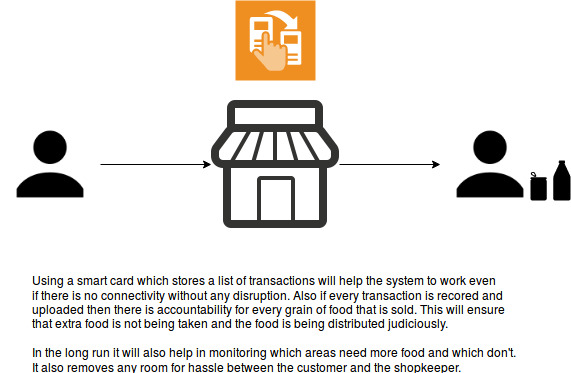
\includegraphics[width=0.8\textwidth]{pds.jpg}}{0.7}
        \end{annotate}
        \caption{A simple visual of CORE PDS\protect\footnotemark}\label{fig:Airbus}
    \end{figure}
    
    \item Standardized measurement units must be used so that the customer gets exactly how much ever they are allocated. There should not be any deceit at the last handshake either. Although it is an infrastructurally demanding order standard food dispensing units can also be made in the long run. This will also help in the storage conditions. 
    
    \item Vending machine type of system will eliminate the need for a shopkeeper (the ethics of killing a job is another question altogether), where a customer will arrive, swipe their card, take a total or a subset of the amount of food allotted to them. There won't be any wastage of food and customers can also be tracked - to see if they are actively using the PDS or not.  

\end{itemize}

\section{Acknowledgements}
\begin{itemize}
    \item I would like to thank my partner (for the previous 2 assignments) and roommate, Kamalnath Polakam, 2015CS10244 for brainstorming with me, which led me to gain better clarity. 
    \item I would like to thank \href{draw.io} for their exceptionally convinient platform to draw charts and figures. All figures have been made using their website. 
    \item I would also like to thank the internet.
\end{itemize}

\section{Bibliography}
\begin{itemize}
    \item \href{https://poorvi.cse.iitd.ac.in/~suban/COP290/pds/reetika-pdsauth.pdf}
    \item \href{http://indiatogether.org/core-pds-smart-system-in-raipur-chhattisgarh-food-security-portability-government}
    \item \href{https://en.wikipedia.org/wiki/Public\_distribution\_system}
    \item \href{http://iseeindia.com/2013/09/10/examples-of-successful-pds/}
    
\end{itemize}


\end{document}